%% This is file `elsarticle-template-1-num.tex',
%%
%% Copyright 2009 Elsevier Ltd
%%
%% This file is part of the 'Elsarticle Bundle'.
%% ---------------------------------------------
%%
%% It may be distributed under the conditions of the LaTeX Project Public
%% License, either version 1.2 of this license or (at your option) any
%% later version.  The latest version of this license is in
%%    http://www.latex-project.org/lppl.txt
%% and version 1.2 or later is part of all distributions of LaTeX
%% version 1999/12/01 or later.
%%
%% Template article for Elsevier's document class `elsarticle'
%% with numbered style bibliographic references
%%
%% $Id: elsarticle-template-1-num.tex 149 2009-10-08 05:01:15Z rishi $
%% $URL: http://lenova.river-valley.com/svn/elsbst/trunk/elsarticle-template-1-num.tex $
%%
\documentclass[preprint,12pt]{elsarticle}

%% Use the option review to obtain double line spacing
%% \documentclass[preprint,review,12pt]{elsarticle}

%% Use the options 1p,twocolumn; 3p; 3p,twocolumn; 5p; or 5p,twocolumn
%% for a journal layout:
%% \documentclass[final,1p,times]{elsarticle}
%% \documentclass[final,1p,times,twocolumn]{elsarticle}
%% \documentclass[final,3p,times]{elsarticle}
%% \documentclass[final,3p,times,twocolumn]{elsarticle}
%% \documentclass[final,5p,times]{elsarticle}
%% \documentclass[final,5p,times,twocolumn]{elsarticle}

%% The graphicx package provides the includegraphics command.
\usepackage{graphicx}
%% The amssymb package provides various useful mathematical symbols
\usepackage{amssymb}
%% The amsthm package provides extended theorem environments
%% \usepackage{amsthm}
\usepackage{tabularx}
%% The lineno packages adds line numbers. Start line numbering with
%% \begin{linenumbers}, end it with \end{linenumbers}. Or switch it on
%% for the whole article with \linenumbers after \end{frontmatter}.
\usepackage{lineno}
\usepackage[round]{natbib}
%% natbib.sty is loaded by default. However, natbib options can be
%% provided with \biboptions{...} command. Following options are
%% valid:

%%   round  -  round parentheses are used (default)
%%   square -  square brackets are used   [option]
%%   curly  -  curly braces are used      {option}
%%   angle  -  angle brackets are used    <option>
%%   semicolon  -  multiple citations separated by semi-colon
%%   colon  - same as semicolon, an earlier confusion
%%   comma  -  separated by comma
%%   numbers-  selects numerical citations
%%   super  -  numerical citations as superscripts
%%   sort   -  sorts multiple citations according to order in ref. list
%%   sort&compress   -  like sort, but also compresses numerical citations
%%   compress - compresses without sorting
%%
%% \biboptions{comma,round}

% \biboptions{}

\journal{Hydrological Procesesses}

\begin{document}

\begin{frontmatter}

%% Title, authors and addresses

\title{Exploring the tropical convective systems formation induced by the  topography structure.}

%% use the tnoteref command within \title for footnotes;
%% use the tnotetext command for the associated footnote;
%% use the fnref command within \author or \address for footnotes;
%% use the fntext command for the associated footnote;
%% use the corref command within \author for corresponding author footnotes;
%% use the cortext command for the associated footnote;
%% use the ead command for the email address,
%% and the form \ead[url] for the home page:
%%
%% \title{Title\tnoteref{label1}}
%% \tnotetext[label1]{}
%% \author{Name\corref{cor1}\fnref{label2}}
%% \ead{email address}
%% \ead[url]{home page}
%% \fntext[label2]{}
%% \cortext[cor1]{}
%% \address{Address\fnref{label3}}
%% \fntext[label3]{}


%% use optional labels to link authors explicitly to addresses:
%% \author[label1,label2]{<author name>}
%% \address[label1]{<address>}
%% \address[label2]{<address>}

\author[1,2]{N. Velasquez}
\author[2, 3]{C.D. Hoyos}

\address[1]{Iowa University, IIHR}
\address[2]{EAFIT university.}
\address[3]{Universidad nacional de Colombia.}

\begin{abstract}
%% Text of abstract
This study evaluates the influence of the orography and its structure over the localization of local convective systems in a portion of the Colombian central Andes. It assumes the orography and its properties as a chain of basins and sub-basins.  At mesoscale, orography has a relevant influence over convective systems, but there is a lack of work at local scale. We identify convective systems, characterized them, and eventually compare them against basins ranging from order 3 to 6.  The comparison is made based on the overlapped area of convective systems and watersheds.  From radar images, we identify convective systems. And obtain basins from a detailed elevation model of 40$m$.  Convective systems exhibit localization and area variations (from less than $2km^2$ to greater than 1000 $Km^2$).  Also, results confirm that there is a preferred localization of convective storms occurrence. And in some regions, convection seems to be profoundly influenced by the interaction of the direction of surface winds and the aspect of some basins, this at multiple scales.
\end{abstract}

\begin{keyword}
Science \sep Publication \sep Complicated
%% keywords here, in the form: keyword \sep keyword

%% MSC codes here, in the form: \MSC code \sep code
%% or \MSC[2008] code \sep code (2000 is the default)

\end{keyword}

\end{frontmatter}

%%
%% Start line numbering here if you want
%%
\linenumbers

%#################################################################
%% main text
\section{Introduction}
\label{intro}

The occurrence of flash floods has caused important human and economic losses for Colombia in the last decade (CITA). And some of the most relevant flash floods are driven by intense convective storms \citep{Maddox1978,Roy2008,Braud2014,Llasat2016}. Just to count two cases, in the year 2015 a deep convective core (DCC) unleashed a flash flood event at Salgar (Antioquia) killing more than 100 people CITA-NICO?, and in 2017, another convective storm killed almost the same amount of people at Mocoa (Putumayo). From historic records we know that flash floods in Colombia tend to happen at the hills of the mountains (CITAS). However, despite the national relevance of this kind of events, there is a lack of regional analysis about them at a proper scale. Also, there are almost no studies that point out the relationship between flash floods and the regional climate conditions.\\

In the Andean region, there are relevant results obtained at mesoscale using TRMM information \citep{Romatschke2010,Romatschke2011a,Mohr2014a,Rasmussen2016c}. Some results suggest significant differences between convective and stratiform systems. For example, \citet{Romatschke2010} highlights the diurnal differences of DCC and WCC (Wide Convective Cores). Also, \citet{Rasmussen2014} describes the occurrence of summer flash floods at the southern Andean foothills caused by deep convective cores. And according to \cite{Zuluaga2015} there is a high occurrence of DCC at the northern Colombian Andean region. In the same study, \citet{Zuluaga2015} describes the diurnal distribution of DCC and WCC cores, and also presents the spatial distribution of the probability location. This described results highlight the relevance that DCC systems has over the Andean region including Colombia.\\

%https://www.tandfonline.com/doi/full/10.1080/02626667.2014.919391
%https://journals.ametsoc.org/doi/full/10.1175/JHM514.1

However, the mentioned works characterize DCC and WCC at the Andean region on a global scale which however is not the proper for the analysis of flash floods CITA. Usually flash floods happen at watersheds with areas below 300 $km^2$ CITA, which makes necessary a detailed characterization of the DCC systems related to them. This detailed characterization could be achieved by using modern land radar systems CITAS, which have been shown to improve storm system analysis CITAs, DCC detection CITAS, and flash floods forecasting and prevention CITAS. For example at CITA shows the success of different early warning systems at the Alps, there are also success cases at the Himalayas CITAS and at the Appalachian mountains CITAS. This evidence suggest the need for a DCC characterization at the Colombian Andean region.\\

In the current work, we present a radar-based characterization of the local convective systems that take place in the central Andean region of Colombia (Figure \ref{fig:localization}).  For this, we use the convective identification algorithm by \cite{Steiner1995}, and based on it, we proposed a novel method for automated identification of ECC (enveloped convective cores) and UCC (unenveloped convective cores). The analysis is based on the images taken by the meteorological radar of the Sistema de Alertas Tempranas de Medellín y el Valle de Aburrá (SIATA) between 2014 and 2016. The presentation of this paper will adopt the following outline. Section \ref{sec:data} describes the region of analysis and the data used for the investigation.  Section \ref{sec:method} explains the procedures done to work with the radar images and the basins.   The results and the discussion are presented in section \ref{sec:results}.  Finally, the conclusions summarize the findings and give suggestions for future research.\\

%#################################################################
%% main text
\section{Data and Methodology}
\label{data_metod}

\subsection{Data}
\label{data}

For the development of the present work, we use the radar information provided by SIATA. The radar is a polarimetric Doppler band C, and is located in the occidental central hill of the watershed (see Figure \ref{fig:localization}). It has a transmission potency of 350 $kW$ with an operational frequency that varies between 5200 and 5700 $MHz$. The beam width reaches near $1^o$, and the maximum operational range oscillates between 500 and 200 $Km$, with an optimum operational range for distances below 120 $Km$ at an inclination of $1^o$.  Additionally, the radar acquires data at a time step of 5$min$ with a reprojected spatial resolution of  128$m$.\\ 

\begin{figure}[t]
\centering
    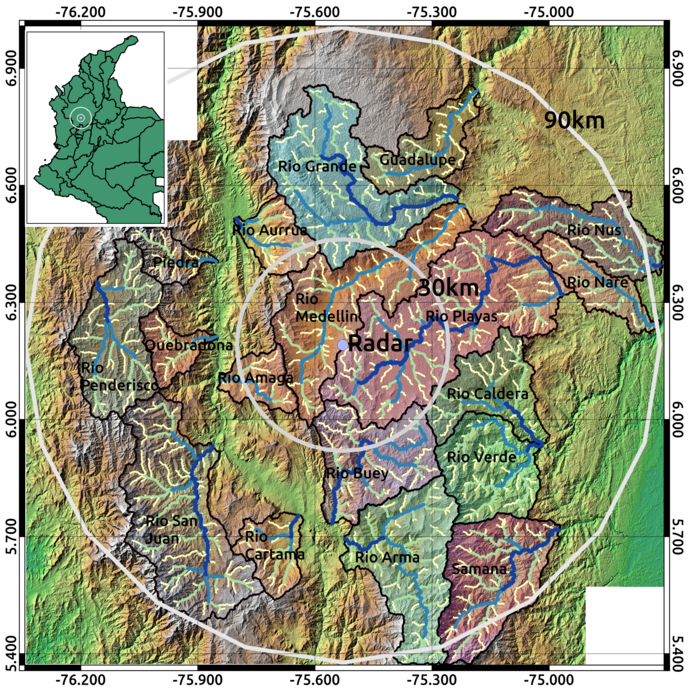
\includegraphics[width=9cm]{Figuras/Analysis_Region.png}
    \caption{Region of analysis, radar localization is presented at the center of the image, gray circles correspond to radar radius of 30 and 90 $Km$ respectively.  Stream orders from 3 to 6 correspond to stream colors (yellow to dark blue).}
    \label{fig:localization}
\end{figure}

The analysis of the radar data is limited to a specific space domain and period.  The radar has information since 2012, but because of poor data quality, we use information taken only between 2014 and 2016.  Also, in order to avoid bright band reflective distortions, the spatial analysis is limited to data obtained below a radius of 90$km$.\\  
 
%!!!!!!!!!!!!!!!!!!!!!!!!!!!!!!!!!!!!!!!!!!!!!!!!!!!!!!!!!!!!!!!!!!!!!!!!!!!!!!!!!!!!!!!!!!!
\subsection{Methodology}
\label{metod}

For the analysis, we extract relevant information of each system recorded by the radar. Depending on the image quality, we classify convective and stratiform systems \citep{Steiner1995}, then sub-classify convective systems into ECC and UCC, and finally assign an ID to each one. At the end of this process, we extract and record some measurements of each system.  At the end, based on this records, we perform a spatio-temporal characterization of the ECC and UCC systems.\\    

\subsubsection*{System classification}

Convective cores classification is done using an implementation of the algorithm proposed by \citep{Steiner1995}.  Our implementation was programmed in Fortran 90, which reduces the processing time, and adds the capability to introduce new functions.  In order to group the measurements of each system, we use a time independent ID for the identified convective (UCC and ECC) and stratiform systems as presented in Figure \ref{fig:SystemClassification}.  The measurements consist of the time and date,  area, maximum longitude, centroid, mean reflectivity and reflectivity deviation.\\      

In the second step of the classification, we identify ECC and UCC systems.  ECC systems correspond to convective systems that are inside stratiform formations.  According to the meteorological conditions of the region, this kind of systems have less energy than UCC, and tend to happen during the morning.  On the other hand, with more energy than ECC systems, UCC systems are likely to occur in the afternoon. This classification is based on the results of the \citet{Steiner1995} classification ($Bin_{class}$).  At $Bin_{class}$ the values that are equal to 1 correspond to stratiform systems, and the values equal to 2 correspond to convective systems. Here we describe our proposed procedure to separate both kinds of convective systems:\\


\begin{itemize}
    \item[1] Convective and stratiform objects are separated into two binaries $Bin_c$ and $Bin_s$ respectively.  $Bin_s$ has values of 1 (stratiform) and 0 (else), $Bin_c$ has values of 2 (convective) and 0 (else), Figure \ref{fig:EnvelopedSeparation} presents an example.

    \item[2] Due to the temporal evolution of the convective cores \citep{Hilgendorf1998,HouzeJr2004,Futyan2007}, UCC systems are likely to be surrounded by a low reflectivity halo that can lead to errors on the classification.  In order to avoid this, $Bin_s$ is eroded by a 3x3 kernel, the result is an eroded binary image of the stratiform systems $BinE_s$ (see Figure \ref{fig:EnvelopedSeparation}b left).  

    \item[3] According to the separation, the regions of $Bin_{class}$ that are equal to 2 are equal to 0 at $BinE_{s}$.  With a filling algorithm, we change the value of these regions to 1, the result becomes a new eroded and filled binary image of stratiform systems $BinEF_s$ (Figure \ref{fig:EnvelopedSeparation}b right).

    \item[4] Then, we obtain a superposition binary ($SupBin_{sc}$) as the sum of $Bin_c$ and $BinEF_s$ (Figure \ref{fig:EnvelopedSeparation}c). For $SupBin_{sc}$, values equal to 2 correspond to UCC systems, and values equal to 3 correspond to ECC systems.

    \item[5] Finally we assign the UCC or ECC classification to each convective system. In order to achieve this, first we identify the cells that correspond to a certain convective system $C_i$ obtained from $Bin_{class}$.  Second, by using steps 1 to 4, the system $C_i$ is identified as a UCC or ECC system depending on the modal value of its cells at the $SupBin_{sc}$ image for time $t$. 
\end{itemize}
\begin{figure}[t]
\centering
    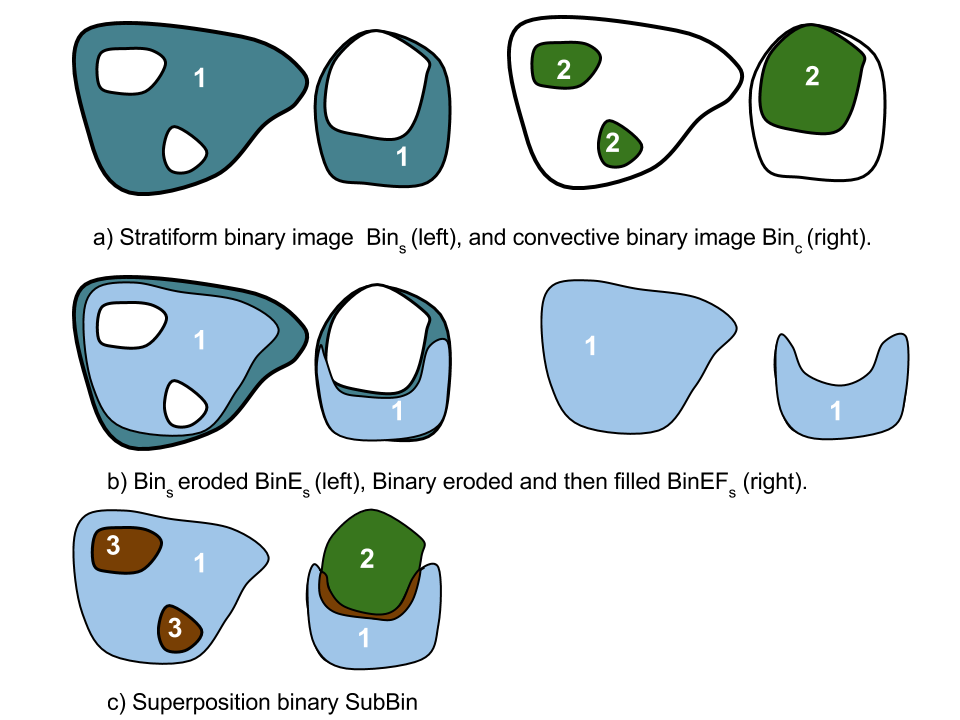
\includegraphics[width=12cm]{Figuras/Enveloped_Stand_Alone_Systems.png}
    \caption{Schematic representation of the proposed methodology used to identify stand alone and enveloped convective systems. a) binaries of convective ($Bin_c$) and stratiform ($Bin_s$) systems are separated, $Bin_c$ takes values of 0 and 2, $Bin_s$ takes values of 0 and 1.  b) $Bin_s$ is eroded, and $BinE_s$ is obtained, then $BinEF_s$ is obtained by filling holes in the binary.  c) $SubBin$ is obtained as the sum of $Bin_c$ and $BinEF_s$, at $SubBin$ values equal to 2 correspond to stand alone convective systems, values equal to 3 correspond to enveloped systems.}
    \label{fig:EnvelopedSeparation}
\end{figure}

At Figure \ref{fig:SystemClassExample} we present an example of the obtained results for an image taken at a random time. The first panel of the figure presents the original image reflectivity.  Panel B presents the  \citet{Steiner1995} classification result or $Bin_{class}$.  For illustrative purposes, panel C shows each system colored depending on their ID. Finally, at panel D we distinguish between ECC (yellow) and UCC (green) systems. 
\begin{figure}[!h]
    \centering
    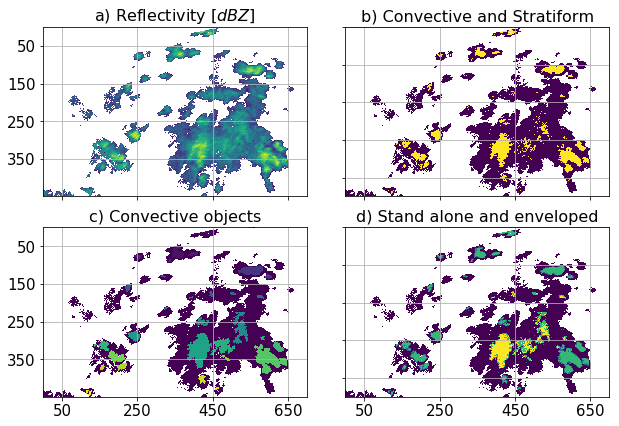
\includegraphics[width=10cm]{Figuras/SystemClass_example.png}
    \caption{Example of classification results.  a) Reflectivity image taken by the radar during October 20 of 2016 at 20:00 P.M local time. b) Convective (yellow) and stratiform (purple) systems identification. c) Convective objects classification by the assignation of an ID for each core. d) Differentiation between ECC (yellow) and UCC  (green)}.
    \label{fig:SystemClassExample}
\end{figure}
After the classification, we take measurements of the morphological and reflectivity characteristics of each system.  These characteristics include the area (in $km^2$), extreme to extreme longitude distribution (in $km$), centroid coordinates ($Lat$ and $Lon$), mean reflectivity ($\mu_{ref}$), and reflectivity deviation ($\sigma_{ref}$). For the estimation of $\mu_{ref}$ and $\sigma_{ref}$ we used $Z$, and then transformed it to reflectivity.  The final step of this characterization consists of the comparison between the described measurements across stratiform, convective, UCC and ECC systems.\\  


\section{Results and discussion}\label{sec:results}
\subsection{Classification validation }
\label{sub:validation}

Considering the records between 2014 and 2017, with the described methodology we manage to classify more than 10000 systems.  The methodology of \citet{Steiner1995} used to identify convective systems is well known, and several works show its performance over the tropical region CITAS.  However, the new methodology presented here to identify ECC and UCC does need a validation that highlights their differences.   For this purpose, we take advantage of the radar operation, which makes three horizontal sweeps and four vertical sweeps every 5 minutes.  In the validation process, we compare randomly detected ECC and UCC systems with their projections over their corresponding vertical profiles.  

%!!!!!!!!!!!!!!!!!!!!!!!!!!!!!!!!!!!!!!!!!!!!!!!!!!!!!!!!!!!!!!!!!!!!!!!!!!!!!!!!!!!!!!!!!!!
\subsection{Characterization}\label{sub:characterization}

%Area and mean reflectivity tend to behave different in convective and stratiform cores (Figure \ref{fig:ConvectiveAreaVsRef}).  The method estimates $\bar{Z}$ (mean reflectivity) as the average of the variable $Z$ for the cells in the system. Then it transforms $\bar{Z}$ into $dBZ$.  And the area was obtained as the sum of the areas of the cells contained in a convective core. According to Figure \ref{fig:ConvectiveAreaVsRef}, some stratiform and convective systems are well differentiated by their mean reflectivity.  Mean reflectivity for stratiform formations 

%oscillates between 5 and 40 $dBZ$. For convective cores, this value oscillates between 30 and 50, with significant less dispersion. Also, there is an important differentiation in the distribution of the plain areas.  While in stratiform systems area oscillate between 0.01 and 13000 $km^2$, at convective systems the area takes values between 0.01 and 80 $km^2$.  Additionally, 80\% of convective systems tend to have areas between 0.8 and 8.5 $km^2$, while 80\% of the stratiform systems area tend to oscillate between 0.8 and 40 $km^2$.\\

%Reflectivity standard deviation ($\sigma_{ref}$) tends to be similar between convective and stratiform systems.  According to the color bar presented at Figure \ref{fig:ConvectiveAreaVsRef}, $\sigma_{ref}$ oscillate in similar values for both kind of systems. However stratiform systems with higher mean reflectivity tend to have a greater value of $\sigma_{ref}$. And convective systems with low mean reflectivity tend to have this similar high value of $\sigma_{ref}$. \\   

At Figure \ref{fig:ConvectiveAreaVsRef} we present an overall comparison between convective and stratiform systems.   The area on the x-axis of the figure corresponds to the projected measured area of each object.  Additionally $\mu_{ref}$ and $\sigma_{ref}$ correspond to the mean and the deviation of the reflectivity of each object considering all its pixels.  Despite the overlap between the two types of systems over the scatterplot, there is a significant separation between the reflectivity and the area histograms (the area is in log scale). This difference can be expressed in terms of the measured $\mu_{ref}$ and area magnitudes. While the mean reflectivity of the convective systems oscillates around 30.5 dBZ, the mean reflectivity of the stratiform systems oscillates around 16 dBZ.   Also, there are differences in the mean value of the areas, which are 24 $km^2$ for convective systems and 47 $km^2$ for stratiform systems.  We present a summary of these results at Table \ref{tab:summary}.

There seem to be some relations among the area, the mean reflectivity $\mu_{ref}$ and the deviation of the reflectivity $\sigma_{ref}$.  For  both types of systems $\sigma_{ref}$  increases and decreases with $\mu_{ref}$. For convective systems with areas below 2 $km^2$ or above 148$km^2$ , $\mu_{ref}$ falls below 35 dBZ and $\sigma_{ref}$ drops down to around 25 dBZ (see Figure \ref{fig:ConvectiveAreaVsRef} ).  With lower values of $\mu_{ref}$, we can observe the same behavior for stratiform systems, with values of $\mu_{ref}$ falling below XX. which show an increase dispersion for higher areas.   

\begin{figure}[!h]
\centering
    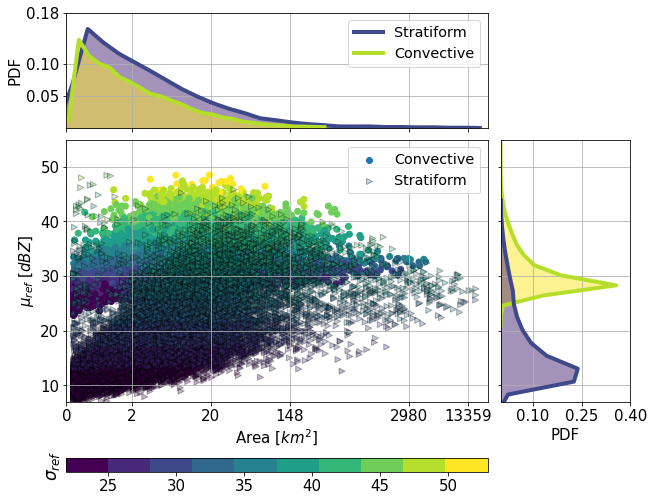
\includegraphics[width=9.7cm]{Figuras/Area_vs_Ref_histos.png}
    \caption{Reflectivity and plain area variations for 10000 random selected systems.  Circles correspond to convective systems, triangles to stratiform systems, color is associated with the variability of the reflectivity inside the system.  Vertical histograms present the PDF for the mean reflectivity for both types of systems.  Horizontal histograms present the PDF for the area for both types of systems.}.
    \label{fig:ConvectiveAreaVsRef}
\end{figure}

\begin{figure}[!h]
\centering
    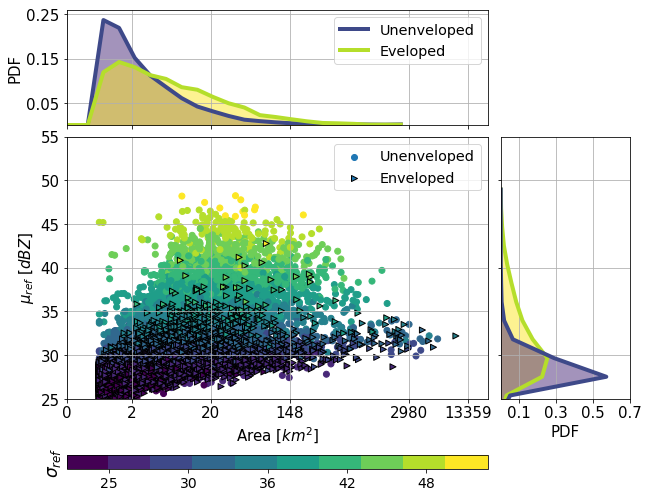
\includegraphics[width=9.7cm]{Figuras/Area_vs_Ref_Conv_In_Out.png}
    \caption{Reflectivity and area comparison for enveloped (triangles) and stand-alone (circles) convective systems. First and second color bars presents the standard deviation for enveloped and stand-alone systems respectively. 80\% of the systems were classified as stand-alone, and 20\% as enveloped.  Vertical histograms present the PDF for the mean reflectivity of both type of systems.}.
    \label{fig:ConvectiveInOutAreaVsRef}
\end{figure}

\begin{table}[t]
\centering
\caption{Summary values of identify systems}
\begin{tabular}{lcccr}
\hline
  \textbf{Property} & \textbf{Stratiform} & \textbf{Convective} & \textbf{Stand alone} & \textbf{Enveloped} \\
\hline
    \textbf{Area} & [$km^2$] & &  \\
    $A_{max}$  & 43000 & 14000 & 14000 & 13200 \\ 
    $A_{mean}$ & 47 & 24 & 30 & 15 \\ 
    $A_{std}$ & 445 & 160 & 180 & 131 \\
    $A_{p10}$ & 1.5 & 1.43 & 1.52 & 1.34 \\
    $A_{p90}$ & 60 & 33 & 43 & 16 \\
\hline
    \textbf{Reflectivity} & [$dBZ$] & & \\
    $R_{max}$ & 40 & 60 & 55 & 46 \\
    $R_{min}$ & 0.26 & 22 & 22 & 22 \\
    $R_{mean}$ & 16 & 30.5 & 32 & 28 \\
    $R_{std}$ & 6.6 & 3.7 & 4.1 & 1.6 \\
    $R_{p10}$ & 10.6 & 27 & 27 & 27 \\
    $R_{p90}$ & 27 & 36 & 38 & 30 \\
\hline
\end{tabular}
\label{tab:summary}
% \belowtable{this table presents a summary of the area and reflectivity variations in stratiform, convective, stand alone and enveloped systems.  Stratiform values where obtained from a sample of about 4 million detected systems.  Convective values where obtained from a sample of about 3 million detected systems.} % Table Footnotes
\end{table}



A similar comparison was done between stand alone and enveloped convective systems. In this case, there are no critical differences between the distributions of the areas of both kind of systems, but there is a difference in the PDF of the mean reflectivity and at $\sigma_{ref}$ (see Figure \ref{fig:ConvectiveInOutAreaVsRef}). Mean reflectivity tend to be less dispersed for enveloped convective systems, with a mean $\sigma_{ref}$ value of 3$dBZ$.  On the other hand, stand-alone systems are more dispersed, with a $\sigma_{ref}$ value of 5 $dBZ$. \\

The described homogenization of the reflectivity and associated diminish of $\sigma_{ref}$, inside the enveloped systems, could be explained by the cycle of life of stand-alone convective cores.  In which usually stand-alone convective cores derive into smaller convective systems surrounded by a stratiform halo \citep{Rasmussen2014}.  Additionally, this feature corresponds too to convective systems formed in the development of a stratiform system. Depending on the case, these enveloped convective systems may or may not be affected by the topography.  Besides, further work is required to differentiate if enveloped systems are the product of the end of a stand-alone system, or if they are a smaller system that travels with a stratiform system.\\


There are differences too in the time of occurrence of stand-alone and enveloped systems. According to Figure \ref{fig:ConvectiveInOut_hour}, stand-alone systems are more likely to happen between 14:00 P.M. and 23:00 P.M.  With important relative peaks at 15:00 and 21:00 P.M.  On the other hand, enveloped systems are more probably to happen between 20:00 P.M. and 05:00 A.M. With peaks at 15:00 P.M and 01:30 A.M, being more significant the peak of the 01:30 A.M. The peak at 15:00 P.M for stand-alone denotes the significant role of the surface heating and the associated deep convection. \\  

\begin{figure}[!h]
\centering
    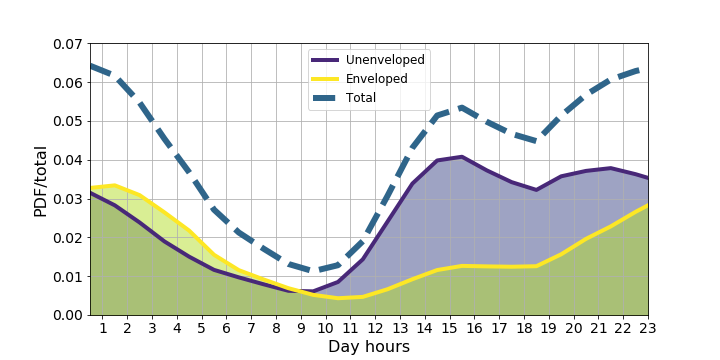
\includegraphics[width=10.3cm]{Figuras/Hitogram_Convective_vs_hour.png}
    \caption{Hourly distribution of the occurrence of total convective (dashed blue), stand-alone (purple) and enveloped (yellow) systems. Stand-alone systems tend to happen during the evening and night.  In the other hand, enveloped systems tend to occur during the morning.}.
    \label{fig:ConvectiveInOut_hour}
\end{figure}

In addition to time differences, there are significant spatial differences in the occurrence of stand-alone and enveloped systems.  There is a trend on the convective spatial localization inside the region of analysis (see Figure \ref{fig:ConvectiveSpatialDistribution}a). The same trend increase for the case of stand-alone convective systems (Figure \ref{fig:ConvectiveSpatialDistribution}b), and decrease for enveloped systems (Figure \ref{fig:ConvectiveSpatialDistribution}c).  Stand-alone convective systems exhibit a strong bound with the topography and therefore with some watersheds.  On the other hand, located in the valleys of analyzed basins, enveloped systems tend to be more dispersed, and seems to be less affected by the topography.\\   

Finally, there is a link between the spatial and temporal localization of convective cores.  The regions of major occurrence vary with the hour of the day. We present this by separate for total convective cores, stand-alone and enveloped ones.  Figure \ref{fig:ConvectiveSpatialDistributionHourly} presents a resume of this spatiotemporal distribution at 6 hours intervals (rows). The column a) corresponds to the total accumulation of convective cores, b) to stand alone and c) to envelop.  How it was presented at Figure \ref{fig:ConvectiveInOut_hour}, in Figure \ref{fig:ConvectiveSpatialDistributionHourly} the time intervals with more convective activity are distributed between 13:00 P.M. and 01:00 A.M, only with significant differences inside the intervals.\\

\begin{figure*}[!h]
\centering
  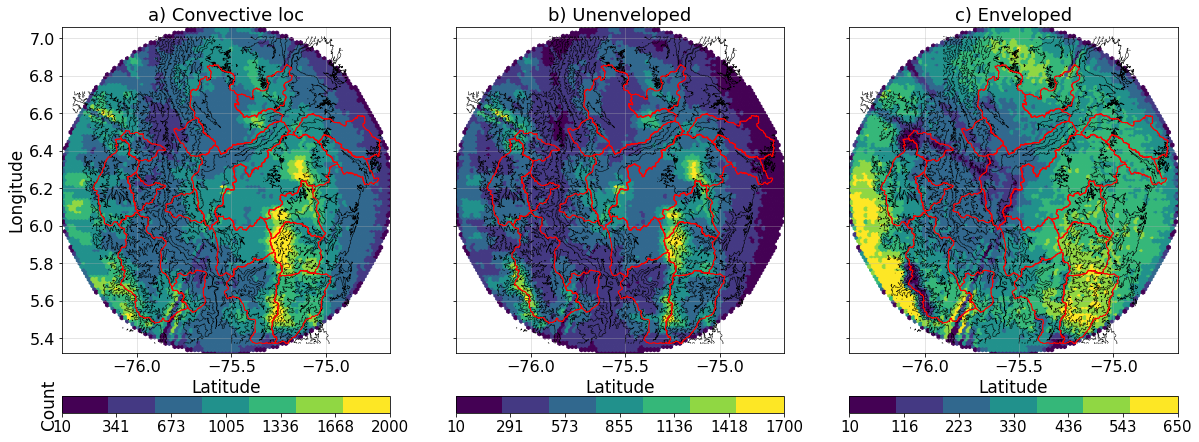
\includegraphics[width=17cm]{Figuras/Localization_conv_evolVsNotEvol.png}
  \caption{2D histogram of convective centroid localization inside the radar region. a) Indiscriminate convective cores localization. b) Stand alone convective cores localization. c) Enveloped convective cores localization.}
  \label{fig:ConvectiveSpatialDistribution}
\end{figure*}

Spatio-temporal variations presented at Figure \ref{fig:ConvectiveSpatialDistributionHourly} show us that there must be more than one mechanism that produces stand-alone and enveloped convective cores.  Between 01:00 A.M and 07:00 A.M. envelop convective cores dominates rainfall production, in this same period stand-alone convective cores do not exhibit a strong presence.  According to this behavior, stratiform systems may produce envelop systems in the morning.  In the next 6 hours period (07:00 A.M - 12:00 P.M), without enough energy for deep convection, and no stratiform entrance, there is no crucial presence of stand-alone and enveloped cores.\\ 

In the other hand, the two periods included between 13:00 P.M and 00:59 A.M. present more convective activity, as is shown at Figure \ref{fig:ConvectiveInOut_hour}. Also, both times present essential differences, while stand-alone cores dominate the period of the evening (13:00 P.M - 18:59 P.M), in the night period (19:00 P.M - 00:59 A.M) there is the presence of both kinds of convective systems.  On the other hand, in the morning (01:00 - 06:59 A.M) stratiform formations may explain envelop cores.  And, the end of stand-alone life cycle may explain night and evening envelop cores.\\

Another difference consists in the localization of convective cores occurrence. During the evening period, there seems to exist more activity in the west region, while in the night period it is focused on the east.  The land-ocean dynamic formed with the pacific \citep{Poveda2004} may produce this variability.\\

Despite the different dynamics that explain the formation of stand-alone and enveloped cores, there seems to be a relation with the topography.  In the accumulated case (Figure \ref{fig:ConvectiveSpatialDistribution}) and in the 6 hour split case (Figure \ref{fig:ConvectiveSpatialDistributionHourly}) there is a preferential localization for convective systems.  The observed relation matches with the boundaries of the basins, and the topography curves (Figure \ref{fig:ConvectiveSpatialDistribution}).\\

\begin{figure*}[!h]
\centering
  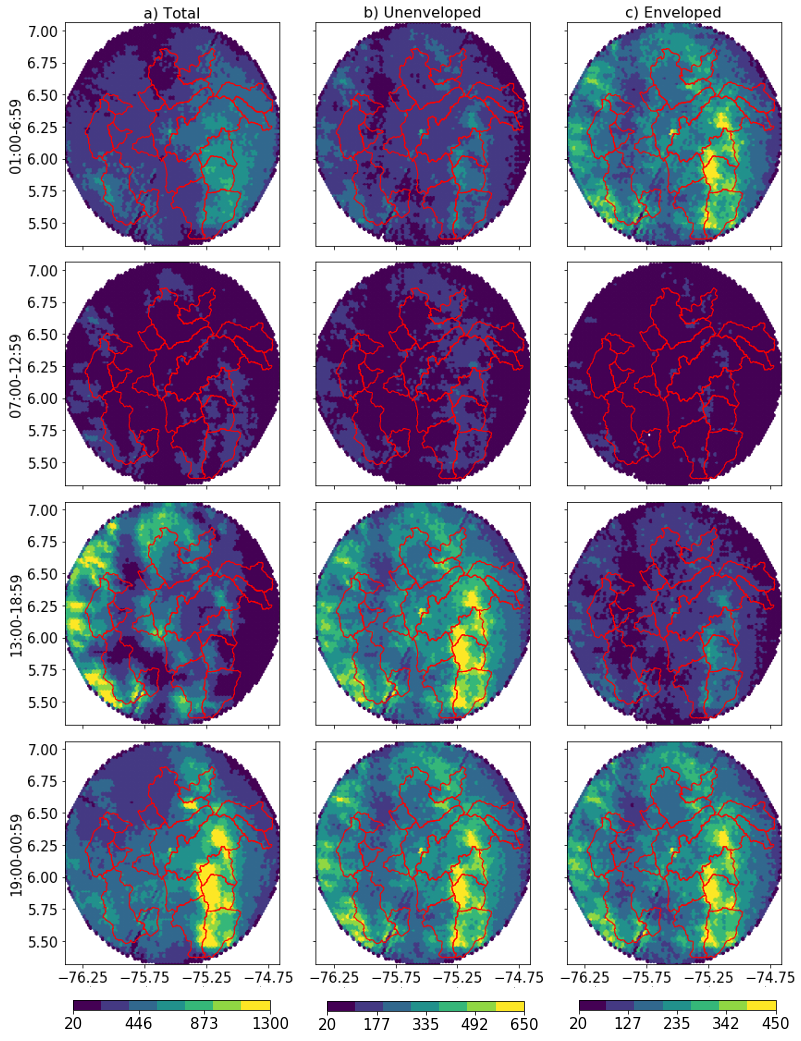
\includegraphics[width=11cm]{Figuras/Localization_conv_evolVsNotEvol_tiempoZoom.png}
  \caption{2D histogram of convective centroid localization inside the radar region varying in periods of 6 hours.  Column \textbf{a} correspond to total convective localization, \textbf{b} to stand alone systems, and \textbf{c} to enveloped systems.  Rows represents accumulations in periods of 6 hours between 01:00 A.M and 19:00 P.M. local time.}
  \label{fig:ConvectiveSpatialDistributionHourly}
\end{figure*}


%\begin{table}[h]
%\centering
%\begin{tabular}{l l l}
%\hline
%\textbf{Treatments} & \textbf{Response 1} & \textbf{Response 2}\\
%\hline
%Treatment 1 & 0.0003262 & 0.562 \\
%Treatment 2 & 0.0015681 & 0.910 \\
%Treatment 3 & 0.0009271 & 0.296 \\
%\hline
%\end{tabular}
%\caption{Table caption}
%\end{table}

%% The Appendices part is started with the command \appendix;
%% appendix sections are then done as normal sections
%% \appendix

%% \section{}
%% \label{}

%% References
%%
%% Following citation commands can be used in the body text:
%% Usage of \cite is as follows:
%%   \cite{key}          ==>>  [#]
%%   \cite[chap. 2]{key} ==>>  [#, chap. 2]
%%   \citet{key}         ==>>  Author [#]

%% References with bibTeX database:

\bibliographystyle{humannat}
\bibliography{bibliography.bib}

%% Authors are advised to submit their bibtex database files. They are
%% requested to list a bibtex style file in the manuscript if they do
%% not want to use model1-num-names.bst.

%% References without bibTeX database:

% \begin{thebibliography}{00}

%% \bibitem must have the following form:
%%   \bibitem{key}...
%%

% \bibitem{}

% \end{thebibliography}


\end{document}

%%
%% End of file `elsarticle-template-1-num.tex'.